%%%%%%%%%%%%%%%%%%%%%%%%%%%%%%%%%%%%%%
% LaTeX poster template
% Created by Nathaniel Johnston
% August 2009
% http://www.nathanieljohnston.com/2009/08/latex-poster-template/
%%%%%%%%%%%%%%%%%%%%%%%%%%%%%%%%%%%%%%

\documentclass[final]{beamer}
\usepackage[scale=1.24]{beamerposter}
\usepackage{graphicx}			% allows us to import images

%-----------------------------------------------------------
% Define the column width and poster size
% To set effective sepwid, onecolwid and twocolwid values, first choose how many columns you want and how much separation you want between columns
% The separation I chose is 0.024 and I want 4 columns
% Then set onecolwid to be (1-(4+1)*0.024)/4 = 0.22
% Set twocolwid to be 2*onecolwid + sepwid = 0.464
%-----------------------------------------------------------

\newlength{\sepwid}
\newlength{\onecolwid}
\newlength{\twocolwid}
\newlength{\threecolwid}
\setlength{\paperwidth}{48in}
\setlength{\paperheight}{36in}
\setlength{\sepwid}{0.024\paperwidth}
\setlength{\onecolwid}{0.22\paperwidth}
\setlength{\twocolwid}{0.464\paperwidth}
\setlength{\threecolwid}{0.708\paperwidth}
\setlength{\topmargin}{-0.5in}
\usetheme{confposter}
\usepackage{exscale}

%-----------------------------------------------------------
% The next part fixes a problem with figure numbering. Thanks Nishan!
% When including a figure in your poster, be sure that the commands are typed in the following order:
% \begin{figure}
% \includegraphics[...]{...}
% \caption{...}
% \end{figure}
% That is, put the \caption after the \includegraphics
%-----------------------------------------------------------

\usecaptiontemplate{
\small
\structure{\insertcaptionname~\insertcaptionnumber:}
\insertcaption}

%-----------------------------------------------------------
% Define colours (see beamerthemeconfposter.sty to change these colour definitions)
%-----------------------------------------------------------

\setbeamercolor{block title}{fg=ngreen,bg=white}
\setbeamercolor{block body}{fg=black,bg=white}
\setbeamercolor{block alerted title}{fg=white,bg=dblue!70}
\setbeamercolor{block alerted body}{fg=black,bg=dblue!10}

%-----------------------------------------------------------
% Name and authors of poster/paper/research
%-----------------------------------------------------------

\title{qooxdoo 3 Part Handling}
\author{Thomas Herchenr\"oder}
\institute{1\&1 Internet AG}

%-----------------------------------------------------------
% Start the poster itself
%-----------------------------------------------------------

\begin{document}
\begin{frame}[t]
  \begin{columns}[t]												% the [t] option aligns the column's content at the top
    \begin{column}{\sepwid}\end{column}			% empty spacer column
    \begin{column}{\onecolwid}
      \begin{block}{Parts}
        \textit{Parts} are a means to \textit{logically} partition a qooxdoo
        application, so that those parts can be loaded \textit{incrementally}
        and \textit{on demand}. Parts are defined by the user through
        configuration entries. The \textit{Generator} uses this configuration to
        distribute class code and resource information across multiple script
        files that are then retrieved via HTTP. The aim is to avoid loading
        of unnecessary code into the browser.
      \end{block}
      \vskip2ex
      \begin{block}{Concepts}
        In order to package the classes of an application (including classes of
        the framework, contribs and any additional libraries) in a way that
        makes for efficient loading, the Generator collects class code into
        \textit{scripts} (.js files). Scripts are grouped into
        \textit{packages}. Scripts of the same package are always loaded
        at the same time (if with multiple HTTP requests). Each \textit{part} is
        implemented by a collection of packages, and a package might be required
        by multiple parts. qooxdoo's \textit{PartLoader} loads all packages for
        a part that has been \textit{require}'d, and have not been loaded yet.
        \begin{figure}
          \begin{center}
            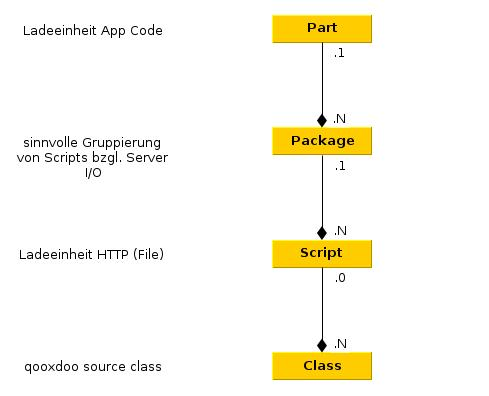
\includegraphics[width=10in]{g_relations.jpg} \\
            \caption{Relations between parts, packages, scripts and classes.}
            \label{fig:corrSubsys}
          \end{center}
        \end{figure}
      \end{block}
      \vskip2ex
    \end{column}

    \begin{column}{\sepwid}\end{column}			% empty spacer column
    \begin{column}{\onecolwid}
      \begin{block}{2-Phase Package Calculation}
        The essence of the realization of parts is the calculation which classes should
        belong to which package. Everything else is derived from that. The
        package calculation process is devided in two steps:
        \begin{itemize}
          \item partition the set of code classes into \textbf{equivalence
            sets} \\
            This means grouping all classes together that are \textit{required by the
            same set of parts}. These groups will be the initial packages. There
            will usually be a large number of them, some with only a few classes.
          \item \textbf{collapsing} (or merging) those packages together, so
            that bigger packages can be fetched with fewer HTTP requests,
            while still preserving that no unnecessary code is loaded into the
            browser.\\
            This will significantly reduce the total number of packages.
        \end{itemize}
      \end{block}

      \begin{block}{Equivalence sets}
        To come up with the equivalence sets for the classes,
        \begin{itemize}
          \item calculate the classes necessary for each part, starting from the
            part's \textit{"include"} config.
          \item for each class in the built, collect the set of parts which
            require this class.
          \item group classes that are required by the same set of parts.
        \end{itemize}
        For example, if you have defined parts "One" and "Two", there will be
        (at most) tree equivalence sets: One set of classes that are required by
        exactly part "One", one set of classes that are required by exactly part
        "Two", and one set of classes that are required by both ["One", "Two"].

        The maximum number of equivalence classes can be expressed as the
        binomail coefficient ${ {N}\choose{k}}$, but for a particular built
        there might be less.
        (TODO).
      \end{block}

    \end{column}

    % column 3

    \begin{column}{\sepwid}\end{column}			% empty spacer column
    \begin{column}{\onecolwid}
      \begin{block}{Conditions for Package Collapsing}
        When collapsing two packages, one is the receiving package to which the
        classes of the second are added, and the other which yields its classes
        and is then removed from the list of packages. For this to succeed, a
        number of constraints have to be observed, or the package calculation
        will result in faulty packages (i.e. packages which will not load
        cleanly in the browser e.g. because of unresolved symbols).
        \begin{itemize}
          \item the receiving package must be loaded for \textit{at least} the
            same parts as the yielding package (i.e. the equivalence class of
            the yielding package must be a subset of that of the receiving
            package)
          \item all load-time dependencies of each class of a package must be
            \textit{within} this package (in load order), or must be in packages
            that are loaded earlier at runtime (TODO)
          \item in all parts where the second package would have been loaded,
            now the first package must be loaded in its place (this might result
            in unnecessary classes being loaded for that part, which is a
            trade-off)
        \end{itemize}
      \end{block}

    \end{column}

    % column 4

    \begin{column}{\sepwid}\end{column}			% empty spacer column
    \begin{column}{\onecolwid}
      \begin{block}{References}
        Some references and a graphic to show you how it's done:
        
        \small{\begin{thebibliography}{99}
        \bibitem{KLPL06} D.~W. Kribs, R. Laflamme, D. Poulin, M. Lesosky, Quantum Inf. \& Comp. \textbf{6} (2006), 383-399.
        \bibitem{zanardi97} P. Zanardi, M. Rasetti, Phys. Rev. Lett. \textbf{79},  3306 (1997).
        \end{thebibliography}}
        \vspace{0.75in}
        \begin{center}
          
\includegraphics[width=3in]{qx.png}
        \end{center}
      \end{block}
    \end{column}

  \end{columns}
\end{frame}
\end{document}
